\chapter{Basic Concepts of Networking}

A computer network, or simply a network, is a collection of computers  interconnected by communication channels that allow sharing of resources and information. Hence a network is a framework in which the connected machines can exchange information. This requirement raises issues like how each machine is individually identified, how the data is exchanged between machine, how the communication is actually conducted etc. Addressing these issues, several networking standards related to addressing schemes, communication protocols, connection paradigms etc. have been developed. Also, based on how a machine acts during its communication gave rise to development of two distinct network models; client server model and peer to peer model.

\section{Addressing}
Every machine connected to the network is uniquely identified by a 4-byte address called Internet Protocol address . This is typically written in dotted quad format like 128.250.25.158 where each byte is an unsigned value between 0 and 255. But a machine in network may be required to provide many services at same time. To distinguish these services, a concept of ports, a logical access point, represented by a 16-bit integer number is used. That means, each service offered by a machine is uniquely identified by a port number.
\section{Protocols}
Communications protocols defines the syntax, semantics for exchanging information in a computer network. Communication Protocols addresses many issues like Data formats and Address Formats for Data exchange, Address mapping and Detection of transmission errors.
Protocols may include signaling, authentication and error detection and correction capabilities.
As far as networking is concerned, all communication protocol can be broadly classified into connection-oriented and connectionless protocol

\subsection{Connection-oriented Protocols}
A connection-oriented protocol is a protocol which established a connection to the receiver and then only send the required data.
The connection path maybe a circuit switched connection, or a virtual circuit connection in a packet switched network.
Connection oriented protocol can be made to deliver data in same order as they were sent and they can also guarantee error free transmission by implementing error detection and correction schemes.
Because they first setup a connection to the host initially, they are substantially slower than there connectionless counter parts.
But they are useful in uninterrupted and secure transmissions.
Some of connection-oriented protocols are:
\begin{itemize}
	\item \textbf{Transmission Control Protocol(TCP)}\\
	TCP provides reliable, ordered delivery of a stream of octets from a program on one computer to another program on another computer. TCP is the protocol used by major Internet applications such as the World Wide Web, email, remote administration and file transfer.
	\item \textbf{Simple Mail Transfer Protocol (SMTP)}\\
	SMTP is an Internet standard for electronic mail (e-mail) transmission across Internet Protocol (IP) networks.
	\item \textbf{Asynchronous Transfer Mode (ATM)}\\
	ATM uses asynchronous time-division multiplexing, and it encodes data into small, fixed-sized cells.
	ATM uses a connection-oriented model in which a virtual circuit must be established between two endpoints before the actual data exchange begins.
	ATM is a core protocol used over the SONET/SDH backbone of the public switched telephone network (PSTN) and Integrated Services Digital Network (ISDN).
\end{itemize}

\subsection{Connectionless Protocols}
Connectionless protocols allow communication between two network end points in which a message can be sent from one end point to another without prior arrangement. The device at one end of the communication transmits data addressed to the other, without first ensuring that the recipient is available and ready to receive the data. Some protocols allow for error correction by requested retransmission. Some connectionless protocols are:
\begin{itemize}
	\item \textbf{Hypertext Transfer Protocol (HTTP)}\\
	HTTP is an application protocol for distributed, collaborative, hypermedia information systems.
	HTTP is the foundation of data communication for the World Wide Web. HTTP is the protocol to exchange or transfer hypertext.
	HTTP functions as a request-response protocol in the client-server computing model. A web browser, for example, may be the client and an application running on a computer hosting a web site may be the server. The client submits an HTTP request message to the server. The server, which provides resources such as HTML files and other content, or performs other functions on behalf of the client, returns a response message to the client. The response contains completion status information about the request and may also contain requested content in its message body.
	\item \textbf{User Datagram Protocol (UDP)}\\
	UDDP is one of the core members of the Internet protocol suite, the set of network protocols used for the Internet. With UDP, computer applications can send messages, in this case referred to as datagrams, to other hosts on an Internet Protocol (IP) network without prior communications to set up special transmission channels or data paths.
	\item \textbf{Internet Protocol (IP)}\\
	Internet Protocol is the principal communications protocol used for relaying datagrams (also known as network packets) across an internetwork using the Internet Protocol Suite responsible for routing packets across network boundaries. It is the primary protocol that establishes the Internet.
\end{itemize}

\section{Network Models}
Based on how communication between two machines in a network is achieved, the mode of communication can be classified as connection oriented and connection-less. In connection oriented mode, two machines must establish an implicit connection between them to communicate where as in connection-less mode, communication progresses without establishing implicit connections.

\subsection{Client-Server Model}
The client/server model is a computing model in which clients request services provided by server. A client does not share any of its resources, but requests a server's content or service function. Clients therefore initiate communication sessions with servers which await incoming requests.
\begin{figure}[htbp]
			\begin{center}
			\setlength{\unitlength}{1cm}
			\begin{picture}(12,5)(0,0)
			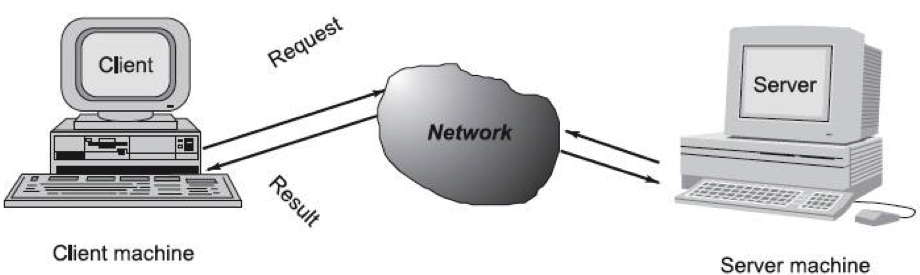
\includegraphics[width=12cm]{./Networking/networking/clientServer.png}
			\end{picture}
	\caption{Client-Server Model}
	\label{ClientServer}
	\end{center}
	\end{figure}
\subsection{Peer-To-Peer Model}
A peer-to-peer (abbreviated to P2P) computer network is one in which each computer in the network can act as a client or server for the other computers in the network, allowing shared access to various resources such as files, peripherals, and sensors without the need for a central server.
P2P is a distributed application architecture that partitions tasks or workloads among peers. Peers are equally privileged participants in the application. Each computer in the network is referred to as a node. The owner of each computer on a P2P network would set aside a portion of its resources - such as processing power, disk storage, or network bandwidth - to be made directly available to other network participant, without the need for central coordination by servers or stable hosts.



